\documentclass[conference]{IEEEtran}
\usepackage{cite}

\IEEEoverridecommandlockouts
% The preceding line is only needed to identify funding in the first footnote. If that is unneeded, please comment it out.
\usepackage{cite}
\usepackage{amsmath,amssymb,amsfonts}
\usepackage{algorithmic}
\usepackage{graphicx}
\usepackage{textcomp}
\usepackage{xcolor}
\usepackage{hyperref}
\usepackage[all]{hypcap}
\def\BibTeX{{\rm B\kern-.05em{\sc i\kern-.025em b}\kern-.08em
    T\kern-.1667em\lower.7ex\hbox{E}\kern-.125emX}}
\begin{document}

\title{Overfitting control with Inverse Cross Entropy loss function (ICE)}

\author{
    \IEEEauthorblockN{Jamshid Bahrami}
    \IEEEauthorblockA{
        \textit{Mazdagineh Street}, Hamadan, Iran \\
        jamshidbahrami@gmail.com
    }
}

\maketitle

\begin{abstract}
In machine learning research community almost all the time researchers use cross entropy between empirical probability function and
target energy function as loss function. In this paper we explore the possibility of doing this in opposite direction in other words
taking cross entropy between empirical energy function and the target probability function. We call resulting loss function Inverse Cross Entropy (ICE).
We prove theoretically and experimentally that this will help us to have control over overfitting, which is not directly possible with former method.
\end{abstract}

\begin{IEEEkeywords}
Loss function, Cross entropy
\end{IEEEkeywords}

\section{Introduction}
The Idea behind the machine learning is that we have a set of inputs
$A=\{a_i\}$ and a set of desired outputs 
$B=\{b_i\}$ corresponding to each of inputs. We suppose that these pairs are well 
representing set of pairs from a real world model,
then our goal is to find a mathematical model $\mathcal{M}$ with two characteristic one that for 
each input it will output corresponding output, we achieve this during the training process
which is explained later, the other is that we expect this model to do the same 
for some unseen samples from real world model after the training.

By passing each $a_i$ through $\mathcal{M}$ we get $\mathcal{M}(a_i)$, but we expect to get $b_i$ the difference between them as you can see in equation \ref{eq:error}
is the error $e_i$, then we represent set of these errors as an empirical distribution \cite{murphy2012machine} with equation \ref{eq:empirical}.
Our goal is to have these errors concentrated around 0, so if we ignore statistics higher than 2 our target distribution is normal distribution with zero mean, to measure how much
we are close to target distribution the common practice is to calculate the cross entropy between these two distributions.
With normal target distribution we end up with equation \ref{eq:crossentropyloss} which is well known mean squared error loss function.
For other loss functions you can get the loss function in similar way for survey on loss functions you can see \cite{wang2020comprehensive}.
Then we try to minimize this loss function with some variant of Stochastic Gradient Descent to train our model.
\begin{equation}
    e_i = \mathcal{M}(a_i) - b_i
    \label{eq:error}
\end{equation}

\begin{equation}
    \sum_{i = 1}^{N}\frac{1}{N}\delta(e-e_i)
    \label{eq:empirical}
\end{equation}

\begin{equation}
    \begin{split}
        L&=-\int(\sum_{i = 1}^{N}\frac{1}{N}\delta(e-e_i)) \log{(\frac{1}{\sqrt{2\pi}\sigma}e^{-0.5\frac{e^2}{\sigma^2}})}  \,de\\
        &=\frac{1}{N}(\sum_{i = 1}^{N}\int\delta(e-e_i)(\log{(\sqrt{2\pi}\sigma)}+0.5\frac{e^2}{\sigma^2})  \,de)\\
        &=\log{(\sqrt{2\pi}\sigma)}+\frac{1}{2N\sigma^2}\sum_{i = 1}^{N}(e-e_i)^2\\
        &\simeq \frac{1}{N}\sum_{i = 1}^{N}(e-e_i)^2\\
    \end{split}
    \label{eq:crossentropyloss}
\end{equation}

\section{Inverse Cross Entropy}

\subsection{Drawback of Cross Entropy}
Ordinary to calculate loss function we put empirical distribution in probability term, $f$ in equation \ref{eq:crossentropy},
while energy term is our target distribution, $g$ in equation \ref{eq:crossentropy}, which is constant, minimum possible value
for this loss function is entropy of $f$, so we can minimize this loss function by minimizing the  entropy of $f$, 
we know from previous section that it is our empirical distribution. Minimum entropy for a distribution is
zero, which is when the distribution is deterministic, it means that we always get same value from distribution.
To minimize the cross entropy with normal distribution this value should be zero. This is  the definition of overfitting.
\begin{equation}
    -\int f(e) \log{g(e)} \,de
    \label{eq:crossentropy}
\end{equation}
\subsection{Inverse Cross Entropy}
We know from previous section that the traditional way of calculating loss function will introduce overfitting term to
our loss function. Based on previous section the natural way of solving this is to switch the terms in equation
\ref{eq:crossentropy}.
\begin{equation}
    \begin{split}
        &-\int(\frac{1}{\sqrt{2\pi}\sigma}e^{-0.5\frac{e^2}{\sigma^2}}) \log{(\sum_{i = 1}^{N}\frac{1}{N}\delta(e-e_i))}  \,de\\
        & = \log{(N)} - \frac{1}{\sqrt{2\pi}\sigma} \int e^{-0.5\frac{e^2}{\sigma^2}} \log{\sum_{i = 1}^{N}\delta(e-e_i)}  \,de\\
        & \simeq - \int e^{-0.5\frac{e^2}{\sigma^2}} \log{\sum_{i = 1}^{N}\delta(e-e_i)}  \,de
    \end{split}
    \label{eq:icrossentropy}
\end{equation}
The equation \ref{eq:icrossentropy} has two calculation drawbacks first it is 
undefined where we do not have samples and in limit it is infinite which is natural
because we are giving infinite value to points that are probable with respect to our
target distribution. The other drawback is that we do not have close solution for the
integral.

To solve these drawbacks we do two things, first we pass our empirical distribution
through a low pass filter, so we have well-defined empirical distribution in all points,
then we approximate the integral by numerical sampling. By doing so we get loss function defined with equation \ref{eq:nicrossentropy}.
\begin{equation}
    \sum_{i=1}^{M}e^{-0.5\frac{e_i^2}{\sigma_1^2}} \log{\sum_{j = 1}^{N}e^{-0.5(\frac{e_j-e_i}{\sigma_2})^2}} 
    \label{eq:nicrossentropy}
\end{equation}

The other way is to just sample calculation points deterministically from target distribution
based on quantiles, in that case we will end up with loss function in 
equation \ref{eq:qnicrossentropy}

\begin{equation}
    -\sum_{i=1}^{M}\log{\sum_{j=1}^{N}e^{-0.5(\frac{e_j-e_i}{\sigma_2})^2}} 
    \label{eq:qnicrossentropy}
\end{equation}

\section{Experiment}
We do curve fitting experiment on model defined in equation \ref{eq:model} where $n$ is a random uniform 
noise in range $(0,  3)$ our proposed model is a 14 layer MLP with relu activation functions.
We choose $\sigma_2=1$ for the experiment.
\begin{equation}
    f(x) = 2x+n
    \label{eq:model}
\end{equation}
Because of the logarithmic nature of our loss function it is sensitive to learning step, so we need an adaptive optimizer,
we use ADAM with $10^{-4}$ learning rate for optimization. In figure \ref{fig:loss} row one 
we have ICE with low variance meaning that we stress on low errors expecting to have more errors
near zero. We see that there is not much of a difference between two loss functions in terms of behavior.
In row two we have widened the variance so after initial steps we are already there, and we  do not 
see significant change in average MSE error. In bottom row we set target distribution to high variance
so in initial steps our model is overfit, and It's trying to diverge from data, so we have increase
in MSE error.

In figure \ref{fig:fit} bottom row we have curve fitting with MSE as we can see our model quickly
starts to fit to data. In rows 2 and 4 we have target distribution with high variance and as it is
obvious from the figure the model is resenting to fit further more to the data. In row two we have the best
fit we have converged to final fitting in initial steps and after that model is almost the same till the end.
In row one we have low variance and our model starts to converge even faster than MSE loss function.

\section{Conclusion}
We presented a novel approach toward calculating model loss function which not only enables us to
have more control over tuning the degree of fitting that we are intended but also lays down 
a well-defined framework for us to design loss functions based on well-defined characteristics.
The code is available through \href{https://github.com/jamshidbb/ice}{https://github.com/jamshidbb/ice}.

\begin{figure}
    \center
    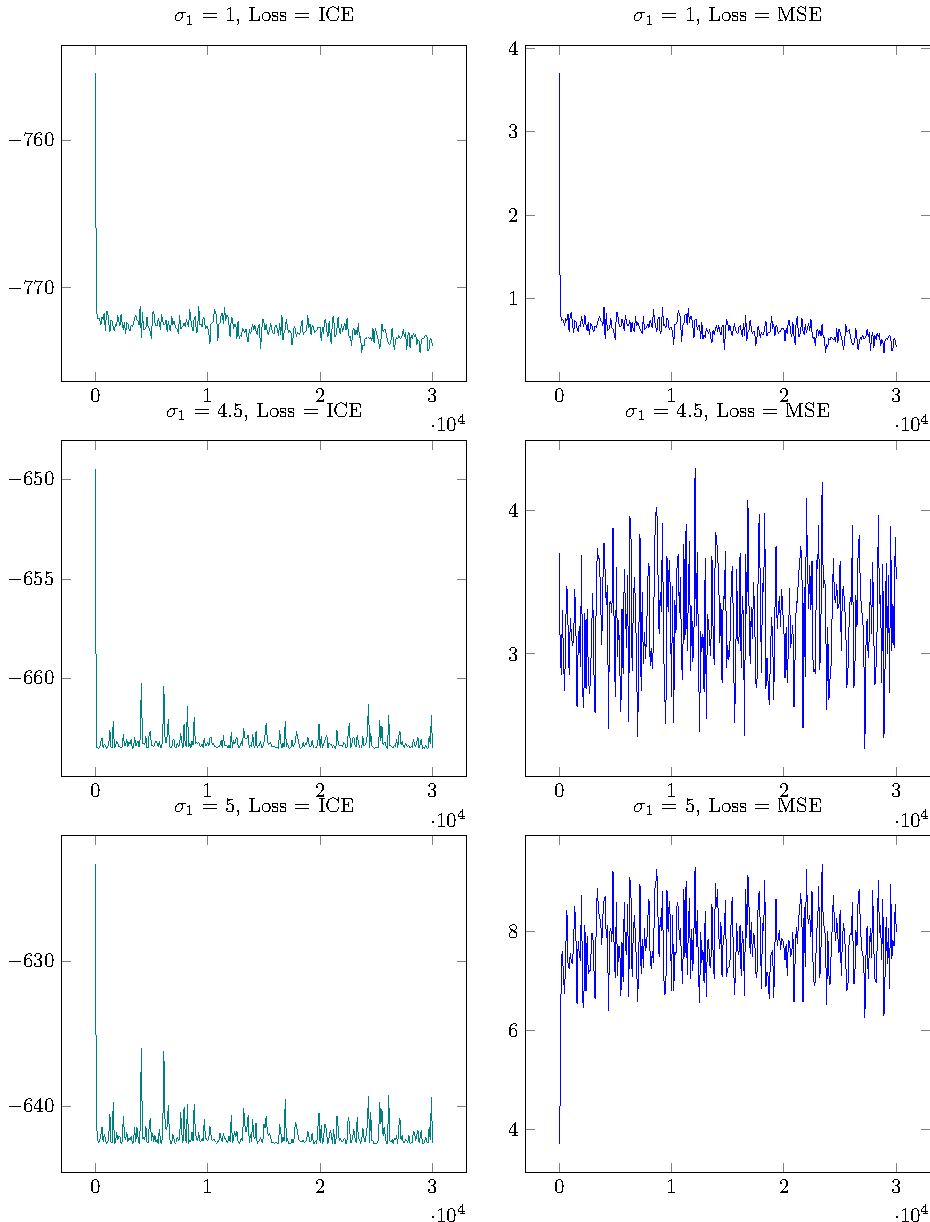
\includegraphics[width=0.70\linewidth]{./fig/losses/out/losses.pdf}
    \caption{
        Loss function for target distribution with different variance.
        Left ICE loss and right MSE evaluated during the training with ICE. In top row we have
        ICE loss with narrow variance, and it is acting like MSE. In bottom row we have ICE
        with wide variance, and it is trying to diverge from data. In middle row we  have 
        moderate variance, and we don't have significant change in MSE.
    }
    \label{fig:loss}
\end{figure}

\begin{figure}
    \center
    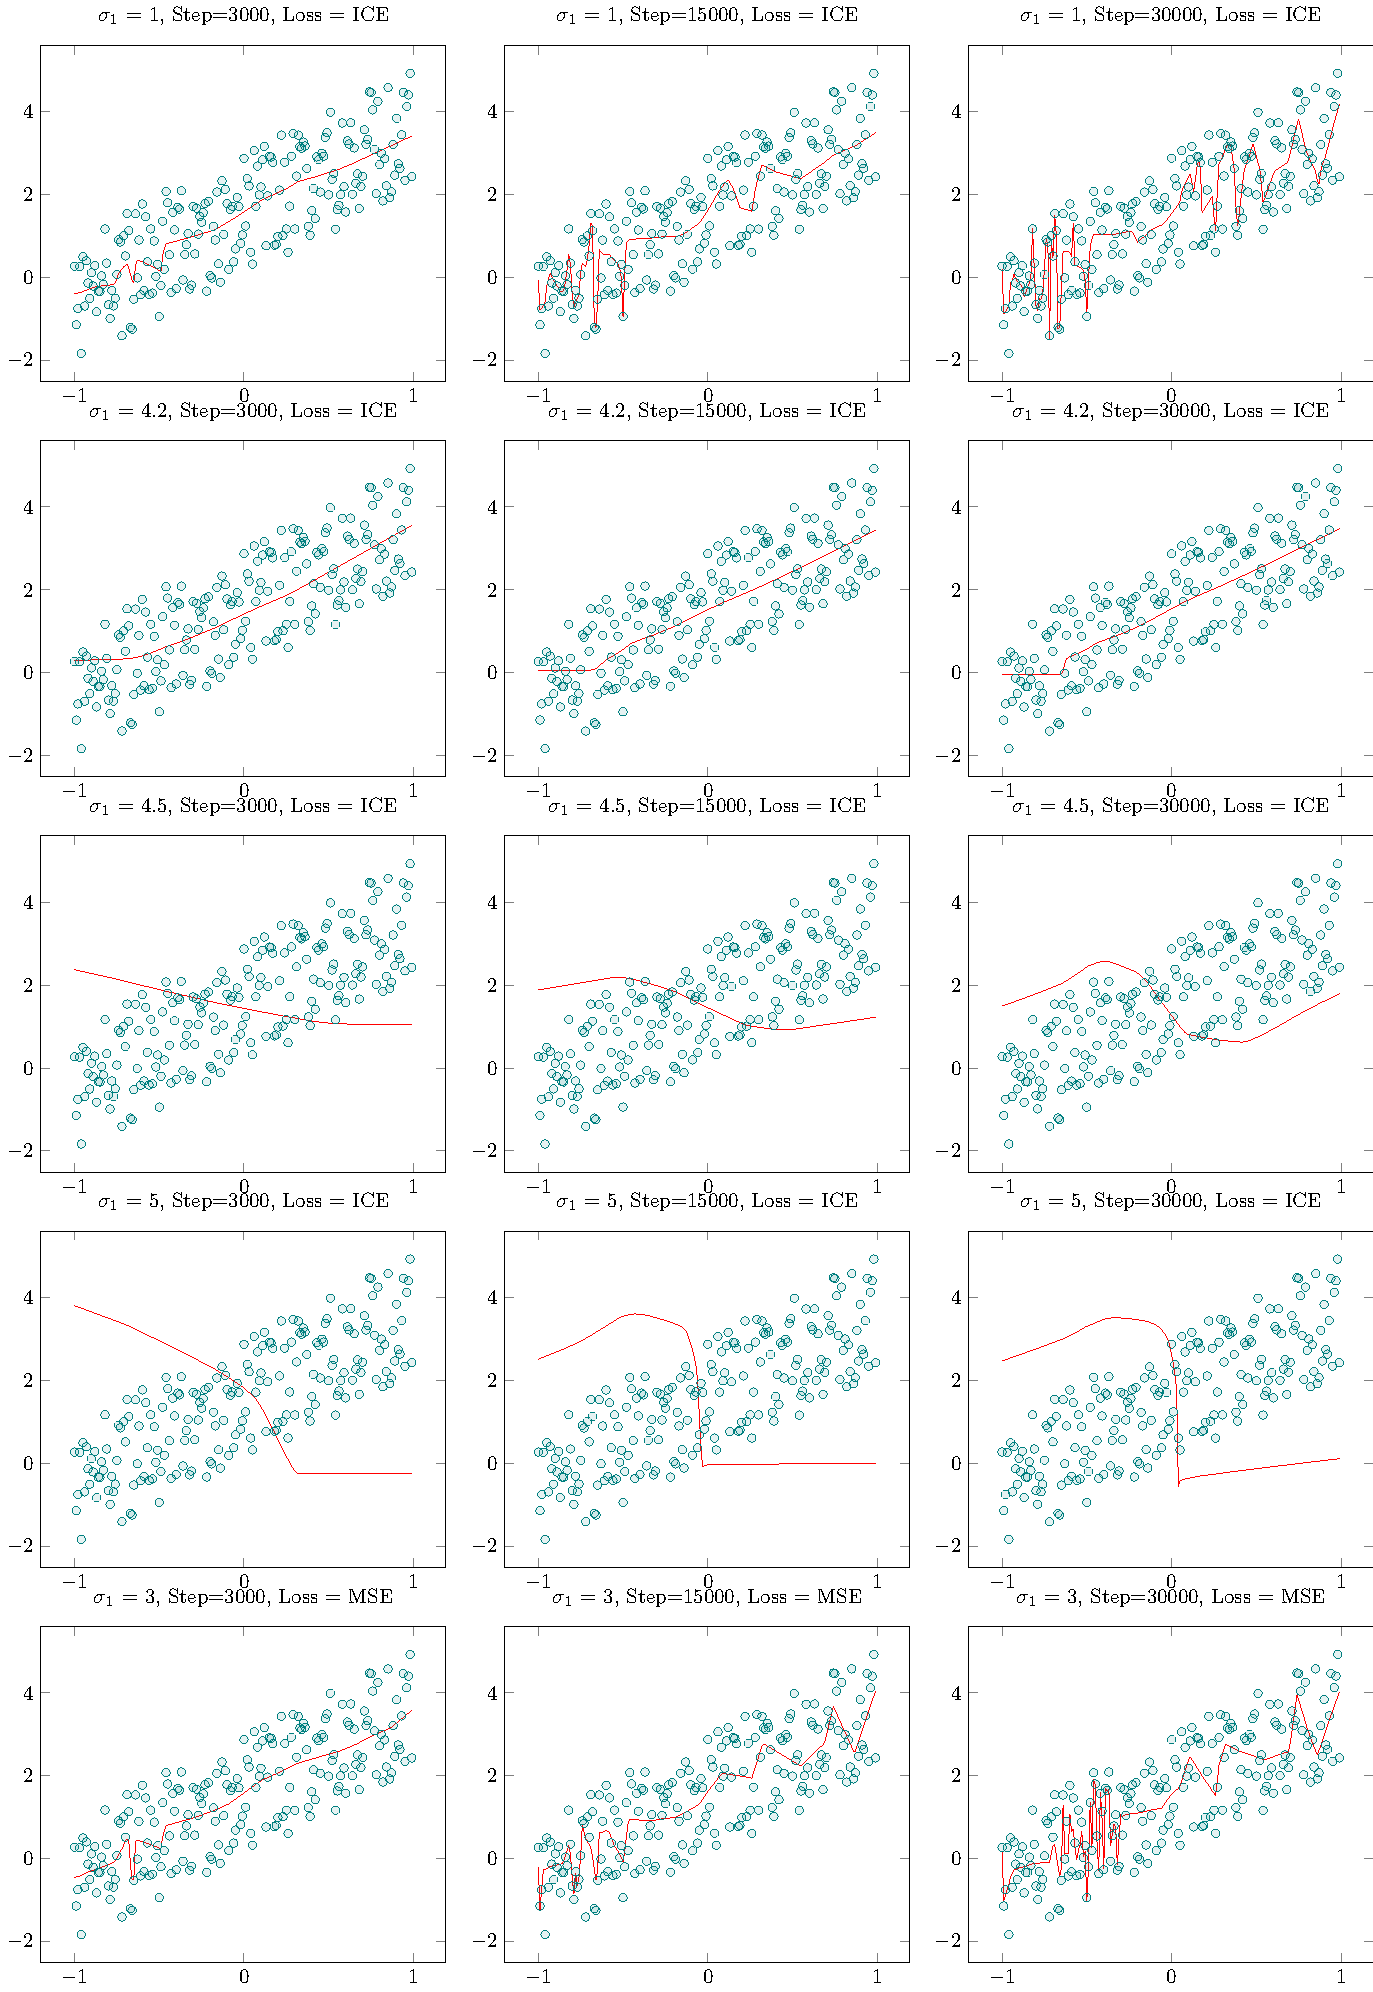
\includegraphics[width=0.85\linewidth]{./fig/expriments/out/exp.pdf}
    \caption{
        Curve fitting experiment. In bottom, we have fitting experiment with MSE error.
        Error variance in ICE are increased from top to bottom and as we can see models tendency toward converging to data is decreased.
    }
    \label{fig:fit}
\end{figure}


\bibliographystyle{IEEEtran}
\bibliography{paper}
\end{document}
